\documentclass[conference]{IEEEtran}
\IEEEoverridecommandlockouts
% The preceding line is only needed to identify funding in the first footnote. If that is unneeded, please comment it out.
\usepackage{cite}
\usepackage{amsmath,amssymb,amsfonts}
\usepackage{algorithmic}
\usepackage{graphicx}
\usepackage{multirow}
\usepackage{array}
\usepackage{textcomp}
\usepackage{xcolor}
\def\BibTeX{{\rm B\kern-.05em{\sc i\kern-.025em b}\kern-.08em
T\kern-.1667em\lower.7ex\hbox{E}\kern-.125emX}}
\begin{document}

\title{TaintBlade: A framework for automated protocol reverse engineering and study of botnet command and control protocols
}

\author{\IEEEauthorblockN{1\textsuperscript{st} Given Name Surname}
    \IEEEauthorblockA{\textit{dept. name of organizatiosn (of Aff.)} \\
        \textit{name of organization (of Aff.)}\\
        City, Country \\
        email address or ORCID}
    \and
    \IEEEauthorblockN{2\textsuperscript{nd} Given Name Surname}
    \IEEEauthorblockA{\textit{dept. name of organization (of Aff.)} \\
        \textit{name of organization (of Aff.)}\\
        City, Country \\
        email address or ORCID}
}

\maketitle

\begin{abstract}
    TODO redact this at the end
\end{abstract}

\begin{IEEEkeywords}
    TODO keywords
\end{IEEEkeywords}

\section{Introduction}
TODO - This section introduces the problem we are dealing with and motivates
the creation of this tool

\section{Background}

TODO - This section goes over the state of the art on analyzing malware
binaries, past work on protocol reverse engineering and available tools.

\section{Design}
TODO - This section covers the general structure of the tool and the different
modules and functionalities implemented.

- Requirements: overview and goals of the tool
- Arch: overview and details of each stage
- Implementation, with repo and how to use

\

In the previous sections, we introduced the issue of automating protocol
reverse engineering and the relevance of this task in the context of the
analysis of malware transmitting malicious communications. In this section, we
will now describe the automated protocol reverse engineering framework, called
\textit{TaintBlade}, that we have developed for tackling this task. Overall,
this tool pursues three main goals: (1) to perform message inference of the
underlying ingress protocol of a program, offering an accurate representation
of its compounding fields and the purpose of each byte; (2) to provide a
complete trace of the activities carried out by the instrumented program,
including a viewpoint into loaded images, child processes, executed routines
and their arguments, therefore helping the analyst with the reversing task,
rathering than just offering a black-box tool; (3) to become a framework usable
not only by malware analysts by offering specific functionalities aimed for
studying malware behaviours, but also by the general public by providing an
intuitive and fully enriched graphical user interface that offers additional
features and enhances cohesion over the data produced by the tool.

\subsection{Architecture overview}

\begin{figure}[htbp]
    \centerline{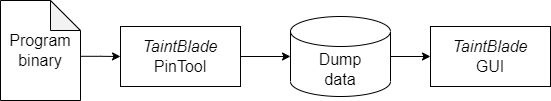
\includegraphics[width=0.9\columnwidth]{images/generalarch.drawio.png}}
    \caption{Example of a figure caption.}
    \label{fig_3_generalarch}
\end{figure}

From a general viewpoint, the functioning of \textit{TaintBlade} is, as shown
in figure \ref{fig_3_generalarch}: (1) the user selects a binary (an
executable) to be traced; (2) the program is executed and instrumented by
\textit{Intel PIN}, using \textit{TaintBlade} as a pintool, which reverses the
protocol of the program; (3) the pintool generates a set of output
\textit{.dfx} dump files and/or a SQLite database with all traced data; (4) the
user can navigate the resulting data by means of \textit{TaintBlade} GUI, which
interacts with the database, or by accessing the output dump files.

The \textit{TaintBlade} pintool is the central component of the framework. It
encompasses all the necessary instrumentation and tracing functionalities
required for the protocol reverse engineering task. At its core, the pintool
utilizes Intel PIN, which provides the instrumentation capabilities. On top of
Intel PIN, \textit{TaintBlade} features a series of \textit{modules} -
collections of components centered on a specific stage of the protocol reverse
engineering task or that offer other additional functionalities intended to
facilitate malware reversing.

As it can be observed in figure \ref{fig_3_archdetailedsteps},
\textit{TaintBlade} comprises six different modules, namely (1) an
instrumentation module which enables the framework to hook on each loaded
image, executed routines and on unique instructions, and to access any register
or memory data; (2) a tainting module featuring a multi-color scheme, which
enables to track the propagation of data at a byte level inside the
instrumented program; (3) a heuristics module that matches executed
instructions with tainted data to a set of heuristics corresponding to specific
operations; (4) a protocol reversing module that constructs a full protocol
from the gathered heuristics; (5) a tracing module that enables to detect the
execution of routines, logging its arguments; (6) and an auxiliary NOPer module
that allows for skipping code sections and to manually modify the program state
at arbitrary points.

Although each module works independently from the others, most of them operate
in a pipeline fashion, where the input of one module depends on that of the one
directly preceeding it. In particular, the instrumentation, tainting,
heuristics and protocol reversing modules work sequentially towards the
protocol reversing task, whilst the tracing and NOPer modules work separately,
offering support features to the tool. We will now study each module
individually and describe how they work internally and the coordination between
them.

\begin{figure*}
    \centerline{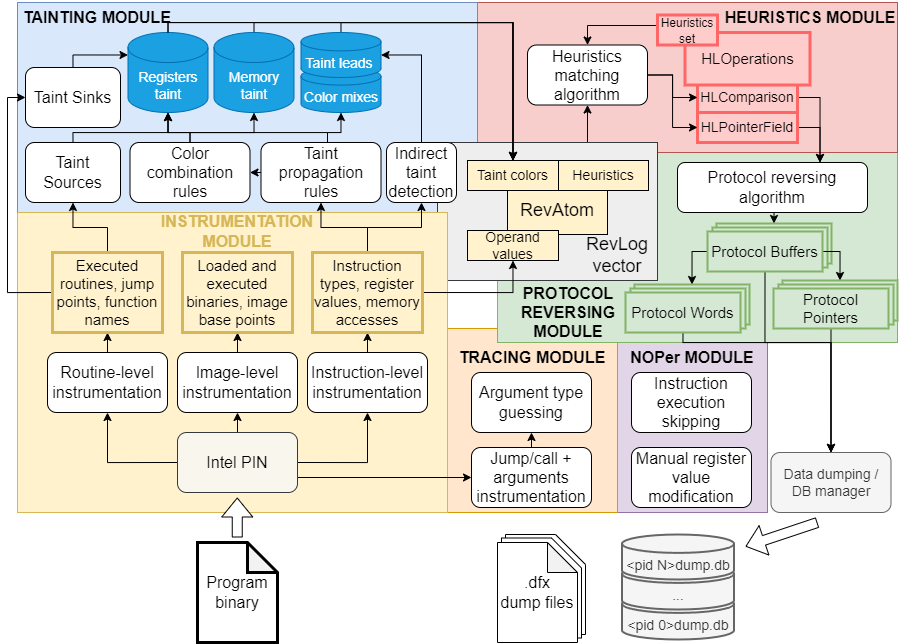
\includegraphics[width=\textwidth]{images/archdetailedsteps.drawio.png}}
    \caption{Example of a figure caption.}
    \label{fig_3_archdetailedsteps}
\end{figure*}

\subsection{Instrumentation module}
The instrumentation module is the central component in the \textit{TaintBlade}
framework and the one that works closer to the assembly code. It utilizes Intel
PIN to instrument the program that is being executed at a triple level:
creating hooks for every loaded program image (e.g. an imported DLL), for every
executed routine (e.g. the \textit{main} function at the program) and for every
executed instruction (e.g. a single call instruction to some other function).

\textbf{Image instrumentation.}
\textit{TaintBlade} only instruments the instructions and routines that are included
in a list known as the \textit{image scope}. This scope is, by default, the main image of the executable
selected to be traced, although the user may select more images to be included via the GUI or
the program configuration files. By instrumenting program images, \textit{TaintBlade} informs the
user of when a new image is loaded - which may be of interest to the user, choosing it to be included
in the scope. This instrumentation also acts as support to other modules - like the NOPer module -, by calculating in
advance the virtual addresses of key instructions (such as those selected by the user to be manually skipped).

\textbf{Routine instrumentation.}
\textit{TaintBlade} instruments any newly executed routine included in the image scope. The instrumentation is double: it instruments
the routine right after it is called and before it returns. This enables
the tool to extract information such as the function and image names, and the memory address of the arguments with which each
function is called and with which it returns. Instrumenting routines is key for supporting the rest of the modules, and it is done in two different ways:

\begin{itemize}
    \item Comparing the name and image of the routine with an internal list of routines.
          The instrumentation of these routines is hardcoded, and therefore the tool
          knows exactly how to parse each of its arguments (the data structures each one
          corresponds to). This type of instrumentation is used from the tainting module,
          which needs to access specific data points in each routine at an specific time
          (either before or after the execution).
    \item Performing a more general instrumentation, without hardcoding the data types.
          As we will explain in section \ref{?}, this is useful for the tracing module,
          which will also attempt to guess the type of arguments later.
\end{itemize}

\textbf{Instruction instrumentation.}
This is the most important instrumentation type since it is the entrypoint for the tainting functionality.
Here \textit{TaintBlade} will examine each executed instruction individually, and
compare it with a list of instructions that the tool is prepared to work with. Table \ref{table:instruction_types_instrumentation_supported}
covers the instruction types currently supported by \textit{TaintBlade}. It must be noted that, for this version of the tool, we have focused
on supporting those instructions that we considered to be more commonly generated by compilers (and thus
more commonly found at any program).

\begin{table}[htbp]
    \caption{Instruction types for which instrumentation is supported}
    \begin{center}
        \begin{tabular}{|>{\centering\arraybackslash}p{2cm}|c|>{\centering\arraybackslash}p{3.5cm}|}
            \hline
            \textbf{Instruction type} & \textbf{Instruction} & \textbf{Description} \\
            \hline
            \multirow{2}{*}{\shortstack{Arithmetic                                  \\ operations}} & ADD & \multirow{2}{*}{\shortstack{Any addition of memory,\\ immediate or register operands}}\\
                                      & SUB                  &                      \\
            \hline
            \multirow{4}{*}{\shortstack{Logical                                     \\ operations}} & AND & \multirow{4}{*}{\shortstack{Any logical operation\\ between memory, immediate\\ or register operands}}\\
                                      & OR                   &                      \\
                                      & XOR                  &                      \\
                                      & SHR                  &                      \\
            \hline
            \multirow{2}{*}{\shortstack{Comparison                                  \\ operations}} &  \multirow{2}{*}{CMP} & \multirow{2}{*}{\shortstack{Comparison between memory,\\ immediate or register operands}}\\
                                      &                      &                      \\
            \hline
            \multirow{5}{*}{\shortstack{Data moving                                 \\ operations}} & MOV & \multirow{5}{*}{\shortstack{Move values and pointers.\\ All types of LEA and MOV\\ instructions are supported}}\\
                                      & MOVSX                &                      \\
                                      & MOVSXD               &                      \\
                                      & MOVZX                &                      \\
                                      & LEA                  &                      \\
            \hline
            \multirow{5}{*}{\shortstack{Control flow                                \\ instructions}} & CALL& \multirow{5}{*}{\shortstack{Any jump, call or return.\\ Supported both near and far\\ relative displacement types}}\\
                                      & JMP                  &                      \\
                                      & JB                   &                      \\
                                      & JBE                  &                      \\
                                      & RET                  &                      \\
            \hline
            \multirow{5}{*}{\shortstack{String                                      \\ manipulation\\ operations}} & SCASB & \multirow{5}{*}{\shortstack{Instructions used for operating\\ with string types, supports\\ iterations with REPNE prefix}}\\
                                      & SCASD                &                      \\
                                      & SCASQ                &                      \\
                                      & SCASW                &                      \\
                                      & REPNE SCASX          &                      \\
            \hline
        \end{tabular}
        \label{tab1}
    \end{center}
    \label{table:instruction_types_instrumentation_supported}
\end{table}

When an instruction is instrumented, \textit{TaintBlade} first checks the type
of instruction by making use of the Intel XED decoder[?] that comes embedded in
Intel PIN. This decoder lets the tool classify the instruction, grouping it
with other instruction types that share the same properties (e.g. every
arithmetic operation is instrumented similarly). Once classified, the tool
analyzes the arguments of the instruction and extracts any needed addresses
and/or values from it. This data will be then used as an input for the tainting
functionality.

\subsection{Tainting module}
\textit{TaintBlade} features a custom multi-color tainting engine for the x86
and x86\_64 architectures, operating at the byte-level. The rationale for this is
that we needed to track and distinguish each byte received from a specific code program point.
By employing multiple colors, we can then gather key information regarding how these bytes
are combined between each other and to know how specific bytes are used inside the program.

This initial version of the tool is fully prepared to work in Windows systems,
although it could be easily extended to work in Linux in a future. It must also
be noted that we decided to develop the tainting system from the ground -
instead of using an existing solution - because we did not find any
implementation of a taint system for x86\_64 Windows machines that included
multi-color taint tracking. We considered well-known engines like libdtf,
Triton or Dytan but, as indicated in table
\ref{table:taining_engines_reason_not_chosen}, we identified certain drawbacks
in each of them.

\begin{table}[htbp]
    \caption{Existing open-source tainting engines, not selected}
    \begin{center}
        \begin{tabular}{|>{\centering\arraybackslash}p{1.5cm}|c|>{\centering\arraybackslash}p{3.5cm}|}
            \hline
            \textbf{Engine}         & \textbf{Characteristics} & \textbf{Drawbacks}                                      \\
            \hline
            \multirow{3}{*}{libdft} & Linux x86                & \multirow{3}{*}{\shortstack{No Windows, x86\_64 support \\ Limited number of colors}}\\
                                    & Multi-color              &                                                         \\
                                    & (max. 8 colors)          &                                                         \\
            \hline
            \multirow{2}{*}{\shortstack{libdft64                                                                         \\ (Angora)}} & Linux x86\_64 & \multirow{2}{*}{\shortstack{No Windows support\\Multi-color not supported}}\\
                                    & Mono-color               &                                                         \\
            \hline
            \multirow{2}{*}{Dytan}  & Linux x86                & \multirow{2}{*}{\shortstack{No windows, x86\_64 support \\ Multi-color not supported}}\\
                                    & Mono-color               &                                                         \\
            \hline
            \multirow{4}{*}{Triton} & Windows, Linux           & \multirow{4}{*}{\shortstack{Multi-color not supported}} \\
                                    & x86, x86\_64,            &                                                         \\
                                    & ARM32, AArch64           &                                                         \\
                                    & Mono-color               &                                                         \\
            \hline
        \end{tabular}
        \label{tab1}
    \end{center}
    \label{table:taining_engines_reason_not_chosen}
\end{table}

We would like to highlight the difficulty of modifying these existing systems
to support our purposes. Adapting an engine to a new architecture requires
creating new taint rules for the new Instruction Set Architecture (ISA).
Moreover, moving from a 32-bit-sized architecture to a 64-bit-sized one
involves additional challenges. One of them is that tainting engines in the x86
architecture usually feature (like in libdft) a shadow memory with the same
size as that of the whole virtual address space (limited to $2^{32}$ bytes in
x86), which tracks the taint state of each byte. This is completely unfeasible
to do in a 64-bit system, since the virtual address space can be up to $2^{64}$
(although processor implementations may reduce this value
\cite{book_practical_binary_analysis_p13}).

Another challenge is the implementation of multi-color taint tracking in a
mono-color system. The introduction of one of such systems involves changing
the taint storage from a bitmap value, where 0=not tainted and 1=tainted, to a
data structure that supports multiple values. Additionally, the number of
possible colors is limited to the capacity of the structure.

Therefore, taking all the previous into account, we decided to create our own
completely new 64-bit-compatible multi-color tainting engine that integrates
with Intel PIN (it relies on the instrumentation module we described
previously).

\textbf{Taint colors and storage.} The tainting module keeps a centralized set
of data structures that store the taint information of the registers and memory of 
a single instrumented process.
Since \textit{TaintBlade} supports both the x86 and x86\_64 architectures, it is not feasiable to
maintain a shadow memory of the process with the color of each byte. Instead, we have
tried to achieve an optimized implementation that pursues two main goals:
\begin{itemize}
    \item Since we cannot shadow all memory in the process, we dynamically generate or destroy
    taint data at runtime, thus giving up on temporal optimization but allowing to taint
    any number of memory addresses.
    \item We expect that taint colors from tainted bytes are frequently combined during 
    program execution. Therefore, we will support an arbitrary number of color combinations,
    improving the design described in section [??reference section showcasing libdft??].
\end{itemize}

Considering the goals described previously, we have developed the tainting engine whose
architecture can be observed in figure \ref{}.



%\section{Implementation}
%NO - This section goes into detail on the algorithms implemented in the tool, including an overview of how the tainting
%engine works and how the heuristics engine and the protocol reversing engine on top work.

\section{Evaluation}
TODO - This section covers multiple test cases, including custom programs that
we will include in our repository that showcase some easy-to-understand cases
we want to show that work, and some others that are real malware found in the
wild.

Goal of the eval first. It's about checking functionality, and checking that we
detect e.g. all commands we know are at the sample

\section{Related work}
TODO decide whether to include this or not - It might fit better in the
background

\section{Conclusion}
TODO - This section offers an overview of the developed tool and the results
obtained over the problem we were trying to solve.

\subsection{Future work \& limitations}

\section*{Acknowledgment}
TODO

\begin{thebibliography}{00}
    \bibitem{b1} G. Eason, B. Noble, and I. N. Sneddon, ``Sample title,'' Phil. Trans. Roy. Soc. London, vol. A247, pp. 529--551, April 1955.
    \bibitem{github_dytan} https://github.com/behzad-a/Dytan
    \bibitem{paper_dytan} https://faculty.cc.gatech.edu/~orso/papers/clause.li.orso.ISSTA07.pdf
    \bibitem{paper_libdft} http://nsl.cs.columbia.edu/papers/2012/libdft.vee12.pdf
    \bibitem{github_libdft64} https://github.com/AngoraFuzzer/libdft64
    \bibitem{github_triton} https://github.com/JonathanSalwan/Triton
    \bibitem{book_practical_binary_analysis} https://terrorgum.com/tfox/books/practicalbinaryanalysis.pdf
    \bibitem{book_practical_binary_analysis_p13} https://www.amd.com/system/files/TechDocs/24593.pdf, Page 13

\end{thebibliography}
\vspace{12pt}

\end{document}

\appendix{}